\documentclass[tikz,border=5pt]{standalone}
\usepackage{tikz}
\usetikzlibrary{arrows.meta, positioning, fit}

\begin{document}

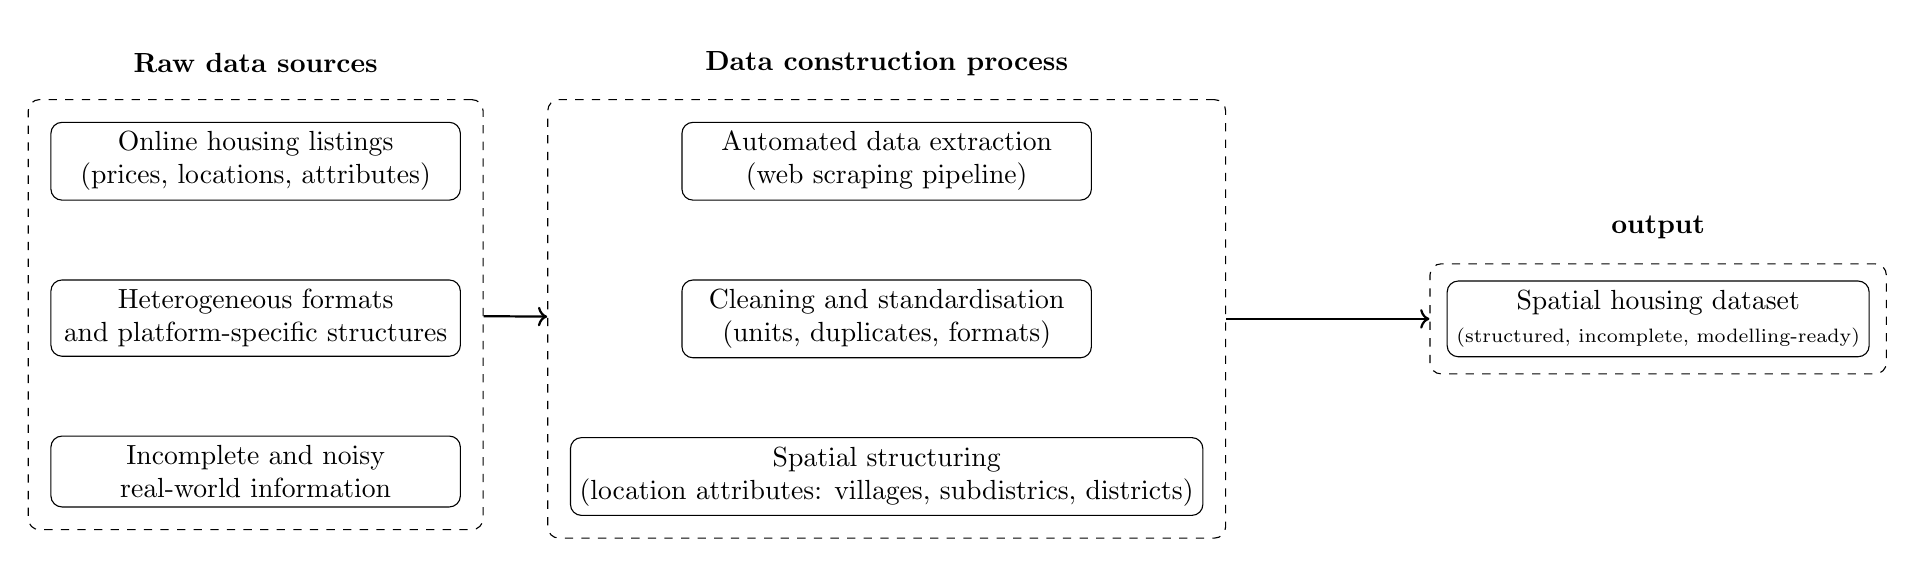
\begin{tikzpicture}[
    every node/.style={
        draw,
        rounded corners,
        align=center,
        minimum width=5.2cm,
        minimum height=9mm
    },
    arrow/.style={->, thick},
    node distance=10mm
]

% ------------------------
% Raw online data (left)
% ------------------------
\node (raw1)
{Online housing listings\\
(prices, locations, attributes)};

\node (raw2) [below=of raw1]
{Heterogeneous formats\\
and platform-specific structures};

\node (raw3) [below=of raw2]
{Incomplete and noisy\\
real-world information};

\node[
    draw,
    dashed,
    rounded corners,
    fit=(raw1)(raw2)(raw3),
    inner sep=8pt,
    label=above:{\textbf{Raw data sources}}
] (rawbox) {};

% ------------------------
% Scraping & processing (middle)
% ------------------------
\node (proc1) [right=28mm of raw1]
{Automated data extraction\\
(web scraping pipeline)};

\node (proc2) [below=of proc1]
{Cleaning and standardisation\\
(units, duplicates, formats)};

\node (proc3) [below=of proc2]
{Spatial structuring\\
(location attributes: villages, subdistrics, districts)};

\node[
    draw,
    dashed,
    rounded corners,
    fit=(proc1)(proc2)(proc3),
    inner sep=8pt,
    label=above:{\textbf{Data construction process}}
] (procbox) {};

% ------------------------
% Constructed dataset (right)
% ------------------------
\node (final) [right=28mm of procbox]
{Spatial housing dataset\\
\scriptsize (structured, incomplete, modelling-ready)};

\node[
    draw,
    dashed,
    rounded corners,
    fit=(final),
    inner sep=6pt,
    label=above:{\textbf{output}}
] (finalbox) {};

% ------------------------
% Arrows
% ------------------------
\draw[arrow] (rawbox) -- (procbox);
\draw[arrow] (procbox) -- (finalbox);

\end{tikzpicture}

\end{document}
